\chapter{实验结果与分析}\label{chapter:experiements}

本章通过实验验证所提出的混合云隐私任务调度模型与算法的有效性。实验通过与多目标优化算法对比,测试本文提出的算法的收敛性与解集质量,还通过与最近的混合云隐私任务调度算法对比,分析不同任务规模、数据隐私需求和加密计算开销对调度结果的影响。研究结果表明,本文方法在提升任务执行效率、数据安全性保障方面均展现出优势,同时成本不劣于其他算法。

\section{实验设置}

为了验证所本文提出的模型和算法的有效性。采用Python 3.13编程语言,基于SimPy 4.1离散事件框架开发混合云仿真系统,运行环境为Windows 10操作系统。为降低随机性对实验结果的影响,通过设置随机数种子控制随机过程,最终结果取10次实验的平均值。本文实现的混合云离散仿真系统,可以反映本文模型中混合云处理隐私数据的特点与流程:私有云作为隐私数据存储与处理的中心;而公有云作为弹性计算资源池,通过安全链路与私有云协同工作。私有云在接收数据处理请求后,根据数据隐私标签、任务计算量等信息,确定公有云与私有云的虚拟机分配方案以及安全策略。

网络拓扑设计参考\parencite{leiPrivacySecurityawareWorkflow2022}中提出的混合云网络模型,公私云虚拟机间直接连接,固定带宽100Mbps。混合云中跨云传输时延为75ms(来自阿里云北京-新加坡地域2025年2月实测)。
% ,详见\url{https://nis.console.aliyun.com/performance/netana}
混合云虚拟机配置参考\parencite{daghayeghiDelayAwareEnergyEfficientTask2024, belgacemMultiobjectiveWorkflowScheduling2022},私有云部署10台异构虚拟机,CPU主频均匀分布于1000-3000 MHz区间。公有云资源配置使用Microsoft Azure Bs v2系列虚拟机 % \cite{DingjiaLinuxXuniji}
% (数据来源:\url{https://azure.microsoft.com/zh-cn/pricing/details/virtual-machines/linux/#bsv2-series-generalpurpose})
,的5种实例类型(3500-56000 MHz),按秒计费,单价区间0.0104-1.1790 \$/h。混合云完整资源配置见表\ref{tab:cloud-resource}。

\begin{table}[htb]
    \centering
    \caption{混合云虚拟机资源配置}\label{tab:cloud-resource}
    \begin{threeparttable}
        \begin{tblr}{lrr}
            \toprule
            类型 & 计算能力 (MHz) & 费用 (\$/h) \\
            \midrule
            私有云 & 1000-3000\tnote{*} & - \\
            公有云B2ts v2 & 3,500 & 0.0104 \\
            公有云B4ls v2 & 7,000 & 0.1470 \\
            公有云B8ls v2 & 14,000 & 0.2950 \\
            公有云B16ls v2 & 28,000 & 0.5890 \\
            公有云B32ls v2 & 56,000 & 1.1790 \\
            \bottomrule
        \end{tblr}
        \begin{tablenotes}
            \raggedleft
        \item[*] 私有云虚拟机的计算能力均匀分布
        \end{tablenotes}
    \end{threeparttable}
\end{table}

% 我们需要修正这一段表述,任务和隐私数据是相互关联的,同时多条任务可以依赖同一条数据。我们考虑两种依赖情况下实验场景,一种是任务与任务均匀依赖数据,此时隐私任务与数据间几乎是1-1对应的。另一种情况是任务依赖一些热点的数据,此时依赖符合Zipf分布,许多任务依赖少数几条隐私数据,且前几条隐私数据的使用频率远高于后几条数据。

% 混合云仿真系统包含一个可配置任务生成器,每次生成200个任务。参考\parencite{kchaouPSOTaskScheduling2022}的研究确定任务与隐私数据间一一对应的关系,每个任务需要一条隐私数据,单个数据规模在10–100 MB均匀分布随机生成,并存储在10台私有云虚拟机的5台上,只有存储了对应隐私数据的私有云虚拟机才能处理任务。任务的数据量是隐私数据的大小,而任务的计算结果固定为隐私数据大小的10%,这反映了通常情况下计算结果大小少于输入数据大小\cite{leiPrivacySecurityawareWorkflow2022}。每处理1bit隐私数据平均消耗一定的CPU周期,具体范围在600至1200区间;而在数据的加解密阶段,也需要消耗CPU周期,具体数值随选择的隐私加密算法有关。每个任务不可抢占,一经分配至虚拟机便独占资源直至完成。
% 参考\parencite{zhuTaskSchedulingMultiCloud2021}的研究,每个隐私数据具有一个最低隐私等级,它限定了数据必须选择高于该等级的隐私加密算法,以满足合规性要求,为了模拟数据的多样性我们设置三类最低隐私等级,其范围分别是-0.1-0.1用于表示低等级隐私数据,0.2-0.9用于表示中等级隐私数据,0.9-1.0用于表示高等级隐私数据,低、中、高三类隐私数据的比例为1:3:1。除了最低安全需求,本文考虑基于数据治理的典型场景,本文设计了三类地域化隐私标签,每类标签有各自的安全策略以满足安全需求,其中中国标签对应网络安全法合规场景、美国标签满足NIST标准要求、欧洲标签符合GDPR合规场景,私有数据的隐私标签比例为1:1:1。

混合云仿真系统包括一个可配置任务生成器,每次生成200个任务。参考\parencite{kchaouPSOTaskScheduling2022}的研究,任务与隐私数据之间存在一一对应关系,即每个任务需要处理一条隐私数据。隐私数据的规模在10–100 MB之间均匀分布随机生成,并存储在10台私有云虚拟机中的5台上。只有存储了对应隐私数据的私有云虚拟机才能处理相关任务。任务的数据量直接由隐私数据的大小决定,而任务的计算结果大小固定为隐私数据大小的10\%,这反映了实际场景中计算结果通常小于输入数据的特点\cite{leiPrivacySecurityawareWorkflow2022}。每处理1bit隐私数据所需的CPU周期在600至1200之间随机分配,数据加解密阶段所需的CPU周期则取决于所选的隐私加密算法。任务具有不可抢占性,一旦分配给某台虚拟机,便独占资源直至完成。

参考\parencite{zhuTaskSchedulingMultiCloud2021}的研究,每条隐私数据具有最低隐私等级,限定了必须选择不低于该等级的隐私加密算法,以满足合规性要求。为模拟数据多样性,本文设置了三种最低隐私等级:低等级隐私数据范围为-0.1至0.1,中等级为0.2至0.9,高等级为0.9至1.0,低、中、高三类隐私数据的比例为1:8:1。

% 此外,本文基于数据治理的典型场景设计了三种地域化隐私标签,分别对应不同的安全策略:中国标签满足网络安全法合规要求,美国标签符合NIST标准,欧洲标签适配GDPR合规场景。私有数据的

% 为确保混合云环境下隐私数据的安全性,本研究构建了符合多国隐私偏好的隐私加密算法组。通过汇总文献\parencite{leiPrivacySecurityawareWorkflow2022, williamAssessmentHybridCryptographic2022, ZhuYingJishitongxinxitongxiaguomiyuguojimimaxingnengbijiao2022, sharifPerformanceAnalysisStream2010}中各类加密方案的加密开销及安全评估指标等研究,以及中、美、欧三国曾经开展的密码标准算法征集活动构建了中国、美国和欧洲的隐私加密算法组。其中,中国标签采用了SM4、SM2及配套SM3算法;美国标签部署了AES、SHA和ChaCha20等加密方案;欧洲标签则选用了HC-128等算法。表\ref{tab:china_encrypt}、表\ref{tab:usa_encrypt}与表\ref{tab:eu_policy}分别展示了各国合规场景下具有代表性的加密方案、加密开销和安全系数指标。

% 为确保混合云环境下隐私数据的安全性,并考虑不同数据所有者细粒度的隐私偏好,本研究构建了包含三个系列密码的隐私加密算法组。通过综合文献\parencite{leiPrivacySecurityawareWorkflow2022, williamAssessmentHybridCryptographic2022, ZhuYingJishitongxinxitongxiaguomiyuguojimimaxingnengbijiao2022, sharifPerformanceAnalysisStream2010}中各类加密方案的加解密开销与安全评估指标研究,并参考中、美、欧三国密码标准算法征集活动的成果,总结出3类隐私加密算法组。具体而言,数据所有者1隐私标签采用了中国商密系列SM4、SM2及其配套的SM3算法;数据所有者2隐私标签部署了美国NIST推荐的AES、SHA和ChaCha20等加密方案;数据所有者3隐私标签则选用了欧洲ENCRYPT密码学竞赛胜出的HC-128等算法。表\ref{tab:china_encrypt}、表\ref{tab:usa_encrypt}与表\ref{tab:eu_policy}分别展示了隐私加密算法及其加解密开销和安全系数指标。

为确保混合云环境下隐私数据的安全性,并满足不同数据所有者的细粒度隐私偏好,本研究构建了一个包含三类加密算法的隐私加密算法组。通过对文献\parencite{leiPrivacySecurityawareWorkflow2022, williamAssessmentHybridCryptographic2022, ZhuYingJishitongxinxitongxiaguomiyuguojimimaxingnengbijiao2022, sharifPerformanceAnalysisStream2010}中各类加密方案的加解密开销与安全评估指标的综合分析,并结合中、美、欧三国密码标准算法征集活动的成果,归纳出了三类隐私加密算法组。具体而言,数据所有者1的隐私标签采用了中国商密标准的SM4、SM2及其配套的SM3算法;数据所有者2的隐私标签部署了美国NIST推荐的AES、SHA和ChaCha20等加密方案;数据所有者3的隐私标签则选用了欧洲ENCRYPT密码学竞赛中胜出的HC-128等算法。表\ref{tab:china_encrypt}、表\ref{tab:usa_encrypt}与表\ref{tab:eu_policy}分别展示了各隐私加密算法组的加解密开销及安全系数指标。隐私标签比例为1:1:1,以反映多样化的数据治理需求。

\begin{table}[htb]
    \centering
    \caption{数据所有者1使用的隐私加密算法组}
    \label{tab:china_encrypt}
    \begin{tblr}{lrrr}
        \toprule
        加密方案 & 加密(CPU周期/bit) & 解密(CPU周期/bit) & 安全系数 \\
        \midrule
        SM4+SM3\cite{ZhuYingJishitongxinxitongxiaguomiyuguojimimaxingnengbijiao2022} & 599.53 & 605.63 & 0.90 \\

        AES+SHA-1\cite{leiPrivacySecurityawareWorkflow2022} & 112.41 & 112.41 & 0.20 \\
        \bottomrule
    \end{tblr}
    \\\hspace*{\fill}\\ % 插入空行
    \caption{数据所有者2使用的隐私加密算法组}
    \label{tab:usa_encrypt}
    \begin{tblr}{lrrr}
        \toprule
        加密方案 & 加密(CPU周期/bit) & 解密(CPU周期/bit) & 安全系数 \\
        \midrule
        AES+ECC+SHA256\cite{williamAssessmentHybridCryptographic2022}& 175.83 & 255.40 & 0.90  \\
        RC4+MD5\cite{leiPrivacySecurityawareWorkflow2022} & 66.15 & 66.15 & 0.26 \\
        \bottomrule
    \end{tblr}
    \\\hspace*{\fill}\\ % 插入空行
    \caption{数据所有者3使用的隐私加密算法组}
    \label{tab:eu_policy}
    \begin{tblr}{lrrr}
        \toprule
        加密方案 & 加密(CPU周期/bit) & 解密(CPU周期/bit) & 安全系数 \\
        \midrule
        HC-128+SHA-1\cite{sharifPerformanceAnalysisStream2010} & 195.75 & 183.20 & 0.60  \\
        RC4+MD5\cite{leiPrivacySecurityawareWorkflow2022} & 66.15 & 66.15 & 0.26 \\
        \bottomrule
    \end{tblr}
\end{table}

\section{评价方案与目标函数介绍}

本文选择了两组对比算法进行性能评估:第一组为任务调度中常见的多目标元启发式优化算法,用于评估NSGA-OW算法的多目标优化性能,包括:
\begin{itemize}
    \item NSGA-II\cite{debFastElitistMultiobjective2002}:经典的多目标进化算法,采用快速非支配排序与精英保留机制,在多种场景中展现了均衡的解集分布和良好的收敛性,常被用于任务调度领域\cite{jafariJointOptimizationEnergy2023}。
    \item SPEA2\cite{daghayeghiDelayAwareEnergyEfficientTask2024}:一种改进的多目标进化算法,引入外部存档机制防止边界解丢失,采用支配强度与k邻近距离分别优化排序精度和密度评估,其ZDT基准测试性能优于传统算法。研究表明,SPEA2在ZDT等基准测试问题上相较于NSGA-II展现出更高的性能。
    \item SMPSO\cite{saifWorkloadAllocationEnergy2023}:多目标粒子群优化算法,在单目标PSO的基础上引入了外部档案机制,缓解了因粒子移动导致的关键边界解丢失问题。相较于传统进化算法,SMPSO具有更快的收敛速度。
\end{itemize}

通过对比上述算法的反世代距离(IGD)以及超体积(HV)指标,可以评估NSGA-OW算法的收敛速度与解集质量。

第二组为混合云隐私任务调度算法,用于评估NSGA-OW算法的任务调度性能,包括:
\begin{itemize}
    \item SPGA\cite{huangImprovedGeneticAlgorithm2023}:通过结合遗传算法和粒子群优化元启发式算法,该算法优化混合云中的任务调度,同时满足隐私需求,提高私有云资源利用率,并确保任务在截止时间前完成。
    \item Min-CAMin\cite{stavrinidesDynamicSchedulingBagsoftasks2021}:Stavrinides提出了一种根据标准差调整完成时间约束以降低混合云成本的隐私任务调度策略,优先降低混合云的开销同时兼顾优化完工时间,并设计了Min-CAMin和Max-CAMin两种启发式算法。经过预实验分析,本文选用Min-CAMin作为对比算法。该算法优先调度最短完成时间的任务,与Max-CAMin相比,能更有效缩短完工时间。
\end{itemize}

通过比较完工时间、安全性和成本指标,可以评估NSGA-OW算法任务调度的性能。

本文提出的NSGA-OW算法的参数设定如下:种群规模为100,迭代次数为1000。在每次迭代中,种群中每个个体会与其编号相邻的个体进行一次交叉操作;交叉操作采用混合交叉算子,其中普通多点交叉算子和虚拟机分块多点交叉算子的使用概率均为50\%。同时,每个个体可能发生变异,变异概率通过公式\eqref{eq:vm-load-prob}动态计算,其最低概率为\(p_0=0.02\),最高概率为\(p_1=0.2\)。

由于其他隐私调度算法未考虑多目标优化,本文采用一种简单的多标准决策(Multi-Criteria Decision Making, MCDM)方法,即伪权重距离方法\cite{sureshMachineLearningBasedPrediction2024},从Pareto前沿中自动提取代表性折衷解,从而实现算法间的性能对比。具体步骤如下:

首先,通过NSGA-OW算法生成非支配解集,每个解的三维目标向量(完工时间、安全性、成本)依据式\eqref{eq:pseudo_weight}进行归一化处理:

\begin{equation}
    \mathbf{p} = \left( \mathrm{norm}\!\left(\text{Makespan}^{(p)}\right), \, \mathrm{norm}\!\left(\text{Security}^{(p)}\right), \, \mathrm{norm}\!\left(\text{Cost}^{(p)}\right) \right)
    \label{eq:pseudo_weight}
\end{equation}

其中,归一化函数定义为\(\text{norm}(x) = (x - x^{\min}) / (x^{\max} - x^{\min})\),\(x^{\max}\)和\(x^{\min}\)分别为目标\(\text{Makespan}^{(p)}, \text{Security}^{(p)}, \text{Cost}^{(p)}\)在非支配解集中的最大值和最小值。归一化后,目标值被映射到区间\([0,1]\),得到伪权重向量\(\mathbf{p} \in [0,1]^3\)。

接着,根据用户偏好定义目标权重参数(本文采用两种权重,分别考虑效率(完工时间)优先\([0.8, 0.2, 0.0]\)和安全性优先\([0.2, 0.8, 0.0]\)),并计算所有非支配解的伪权重与目标权重间的欧氏距离。最终选取距离最小的解作为折衷解,分别将其命名为NSGAOW-1(效率优先)和NSGAOW-2(安全优先)。

本节设计了算法性能评价方案。首先,通过对比NSGA-OW与三种经典多目标优化算法(NSGA-II、SPEA2、SMPSO),验证其在多目标优化方面的性能;其次,对比两种混合云隐私任务调度算法,以完工时间(式\eqref{eq:makespan})、安全性(式\eqref{eq:security})及成本(式\eqref{eq:cost})为评价指标,评估隐私任务调度性能。采用伪权重法从Pareto前沿解集中选取效率和安全性两种偏好的折衷方案,分别命名为NSGAOW-1和NSGAOW-2,为混合云任务调度提供多样化解决方案。

\section{多目标优化的收敛性与非支配解集质量分析}

为评估多目标优化算法的性能,本文选取反转世代距离(Inverted Generational Distance, IGD)和超体积(Hypervolume, HV)指标对解集的收敛性及多样性性能进行分析。统一采用的OW-FF以充分利用虚拟机的资源空闲时段,通过对比NSGA-OW与NSGA-II、SPEA2和SMPSO三种元启发式算法的实验结果,可验证改进算法的多目标优化性能。实验结果如图~\ref{fig:gd}和图~\ref{fig:hv}所示。

\begin{figure}[htb]
    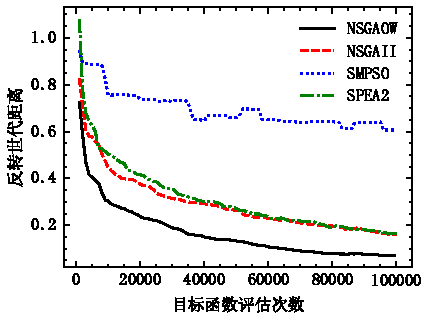
\includegraphics{img/igd.pdf}
    \caption{多目标优化算法收敛速度比较}\label{fig:gd}
\end{figure}
\begin{figure}
    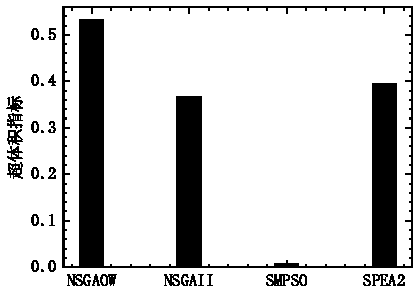
\includegraphics{img/hv.pdf}
    \caption{多目标优化算法超体积指标}\label{fig:hv}
\end{figure}

实验结果表明,NSGA-OW在收敛性能和全局解集质量上均优于对比算法。在收敛速度方面,NSGA-OW仅需30000次函数评估即可达到IGD值0.19的水平,而NSGA-II与SPEA2需83000次和79000次评估才能达到同等收敛程度;在解集质量方面,NSGA-OW的HV指标为0.53,分别较SPEA2和NSGA-II提升35.9\%与43.2\%。这种性能提升主要来自针对混合云任务调度问题改进的遗传算子设计。虚拟机分块多点交叉算子以虚拟机为单位交换任务分配方案,保留了优质分配模式的完整性,而负载动态变异算子通过动态调整变异概率进一步提升了搜索效率和精度。值得注意的是,SMPSO在本文场景中表现不佳,这是因为尽管其采用了外部存档和拥挤机制来优化多目标搜索性能,但S作为群优化算法,基于连续空间的速度更新规则难以适应本文离散优化问题。实验结果验证了NSGA-OW多目标优化算法在求解本文多目标优化问题上相比其他算法具有良好的收敛速度与解集质量。

\section{任务量和数据规模对算法的影响}

本节实验分为任务量和数据规模两个维度进行性能评估。在任务量对比实验中,隐私数据量服从[10-100] Mbit的均匀分布,任务总数分别设置为100、200、300、400和500个任务,重点考察任务数量维度变化对调度性能的影响规律。在数据规模对比分析中,保持任务总数为200个恒定,通过设定隐私数据量的均值分别为10、30、50、70和90Mbit构建不同测试场景,其中每个场景的数据量以对应的均值中心±5 Mbit均匀分布展开(例如均值30 Mbit时数据量分布在[25,35] Mbit范围内均匀分布),旨在量化分析单任务数据规模变化对调度目标的影响特征。

\begin{figure}[htb]%
    \subfloat{
        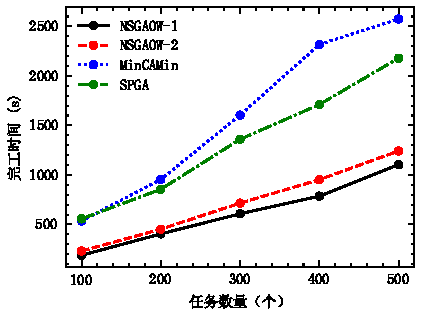
\includegraphics{img/task_amount_vs_makespan.pdf}
        \hfill
        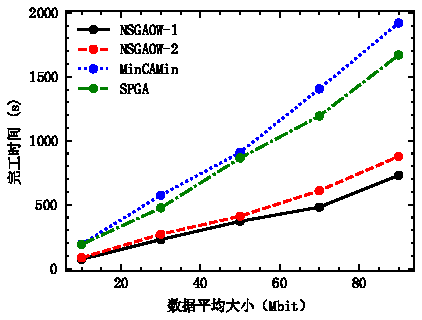
\includegraphics{img/data_size_vs_makespan.pdf}
    }
    \caption{任务数量与数据规模对混合云完工时间的影响}\label{fig:task_amount_vs_makespan}
\end{figure}

% 需要将“我们”改成“本文”

首先,本文分析任务数量与数据规模对完工时间的影响。从实验结果可以看出,随着任务数量或数据规模的增加,完工时间均呈上升趋势,这与预期一致。例如,当任务数量为200(数据量均值为55 Mbit)时,完工时间为452.18秒,与数据规模实验中50 Mbit场景的410.47秒(NSGAOW-2)接近,验证了实验环境的可复现性。
接下来,NSGAOW-1和NSGAOW-2在两种实验环境中均表现出最优的完工时间性能。例如,当任务数量为500时,NSGAOW-1的完工时间为1103.69秒,显著低于MinCAMin的2574.63秒和SPGA的2178.51秒。这一优势主要源于NSGAOW算法在设计中对公私云协作和虚拟机空闲时段的优化,提高了资源利用率。相比之下,对比算法SPGA和MinCAMin由于采用单目标优化策略,SPGA以私有云利用率,而MinCAMin以混合云成本为首要优化目标,未能最优化完工时间。其完工时间在500任务时分别为2178.51秒和2574.63秒,均显著高于NSGAOW系列算法,表明间接优化完工时间的效果不及直接优化多目标的NSGAOW算法。
此外,本文发现NSGAOW-2的完工时间普遍高于NSGAOW-1,例如在任务数量为500时,NSGAOW-2的完工时间为1242.01秒,而NSGAOW-1为1103.69秒。这是由于NSGAOW-2优先考虑安全性优化,牺牲了部分完工时间。然而,得益改进的公私云协作模型和多目标优化特性,NSGAOW-2仍优于其他算法(如MinCAMin和SPGA)。例如,在数据规模为90 Mbit时,NSGAOW-2的完工时间为877.04秒,低于SPGA的1669.69秒。

\begin{figure}[htb]
    \subfloat{
        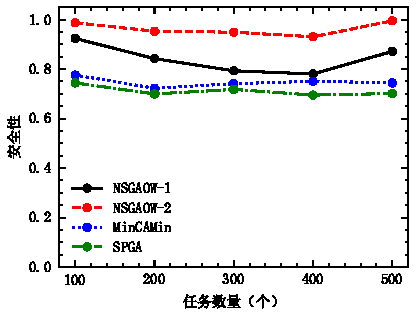
\includegraphics{img/task_amount_vs_security.pdf}
        \hfill
        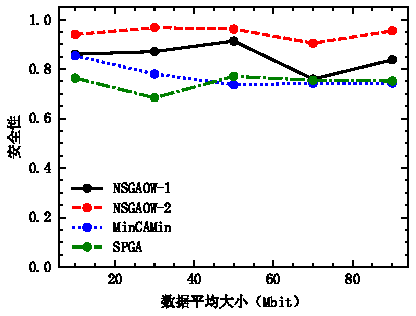
\includegraphics{img/data_size_vs_security.pdf}
    }
    \caption{任务数量与数据规模对混合云安全性的影响}\label{fig:task_amount_vs_security}
\end{figure}

本文分析了任务数量与数据规模对安全性的影响,发现NSGAOW-2的效果优于其余三种策略,而NSGAOW-1的安全性不劣于对比算法。例如,在任务数量为500时,NSGAOW-2的安全性达1.00,而MinCAMin和SPGA分别为0.74和0.70,验证了NSGAOW算法在优化本文提出的量化安全性指标中表现出色,更好地保护了隐私数据安全。

同时,尽管NSGAOW-1更倾向于通过公私云协作优化完工时间,但其安全性仍不劣于对比算法。例如,在任务数量为100时,NSGAOW-1的安全性为0.92,高于MinCAMin的0.78和SPGA的0.74。这种表现得益于NSGA-OW的多目标优化方法:只有安全性、完工时间与成本至少有一方占优的非支配解才可能成为候选调度方案。此外,本文采用伪权重法(权重为[0.8, 0.2, 0.0])选择调度方案,虽然偏向完工时间优化,但仍兼顾了安全性,因此NSGAOW-1在安全性上不劣于对比算法。

本文还发现,随着任务数量增加,NSGAOW-1与NSGAOW-2的安全性差距扩大。例如,在任务数量为100时,两者安全性分别为0.92和0.99,差值为0.07;而在任务数量为500时,两者安全性分别为0.87和1.00,差值扩大至0.13。这种现象的原因是:随着任务数量增加,私有云负载上升,NSGAOW-1倾向于通过更多的公私云协作降低完工时间,从而牺牲部分安全性以提升任务执行效率。这反映了NSGAOW算法能够为用户提供多样化的调度方案,满足不同的优化需求。

在数据量较大时,NSGAOW-1 的安全性表现有所下降。例如,在数据量为70 Mbit时,NSGAOW-1的安全性为0.76,与 MinCAMin 的0.74和 SPGA 的0.75接近。这一现象的主要原因是:高数据量场景时,隐私加密算法的加密时间较长,导致无法充分利用卸载窗口处理其他任务,因此NSGAOW-1倾向于选择开销较低但安全性较弱的加密算法。这也体现了数据量对算法调度方案的影响。

\begin{figure}[htb]
    \subfloat{
        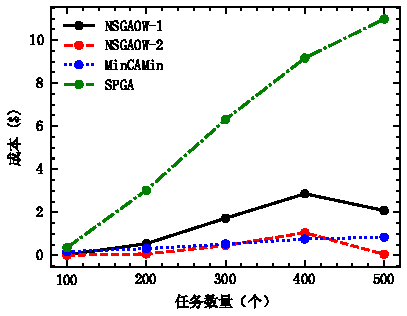
\includegraphics{img/task_amount_vs_cost.pdf}
        \hfill
        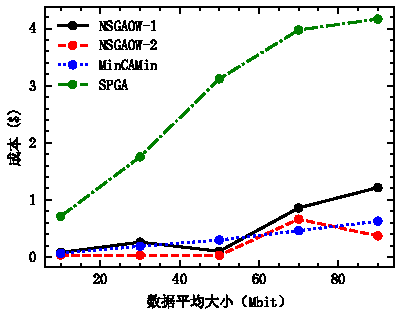
\includegraphics{img/data_size_vs_cost.pdf}
    }
    \caption{任务数量与数据规模对混合云成本的影响}\label{fig:task_amount_vs_cost}
\end{figure}

在成本方面,实验数据显示NSGAOW-2和MinCAMin表现最优,在数据量为90 Mbit时分别为0.37元和0.63元。这是因为MinCAMin的优化目标只有成本,其通过第一轮循环筛选满足完成时间约束的虚拟机,在第二轮循环中从中选择成本最低的虚拟机。NSGAOW-1同时优化安全性与成本,且倾向于选择安全性较高的调度方案,而私有云独立处理的安全性最高。由于私有云成本固定,选择高安全性方案也间接降低了成本。
而SPGA虽然通过最大化私有云资源利用率理论上可以降低成本,但未考虑优化公有云成本,导致其倾向于租用更多公有云虚拟机以满足截止时间需求,因此成本较高。例如,在数据量为90 Mbit时,其成本为4.17元。相比之下,NSGAOW-1优先优化完工时间,虽然会租用更多公有云虚拟机增加成本,但其成本为1.22元,低于SPGA的4.17元。

本节实验表明,NSGA-OW算法具有良好性能。其中,优先效率优化的NSGAOW-1策略在任务量为200数据规模为 [10, 100] Mbit 的均匀分布时,完工时间为404.43秒,相较于对比算法SPGA(855.07秒)降低了52.7\%。而优先安全性优化的NSGAOW-2策略在安全性指标上同样表现优异,其安全性为0.95,相较于对比算法MinCAMin(0.72)提升了31.9\%。同时NSGA-OW在成本上不劣于对比算法。

\section{数据隐私需求对算法的影响}

本小节研究隐私数据特性对调度算法性能的影响,分析数据的最低隐私需求、数据热点及存储分布对完工时间的影响。在最低隐私需求的影响实验中,本文固定数据的范围是5-10Mbit,本文通过调整任务的最低隐私需求范围,设计了三种不同的场景:场景2为低隐私需求占10\%、中隐私需求占80\%、高隐私需求占10\%(原始配置);场景1为低隐私需求占70\%、中隐私需求占30\%(整体隐私需求较低);场景3为中隐私需求占20\%、高隐私需求占80\%(整体隐私需求较高)。

\begin{figure}[htb]
    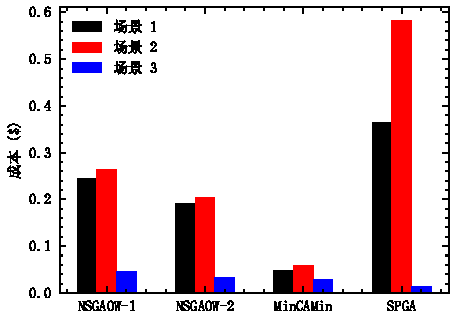
\includegraphics{img/min_secu_vs_cost.pdf}
    \caption{不同隐私需求场景对成本的影响}
\end{figure}

通过对不同安全性场景下算法成本表现的分析,本文发现:

在场景2中,四类调度策略成本均最高,例如NSGAOW-1成本为0.26元,SPGA成本为0.46元。这是因为场景2包含最多中等隐私需求的数据,这类数据可以通过跨云协作处理,但必须使用高等级隐私加密算法,导致消耗更多公有云资源,使成本增加。

从场景1到场景2,NSGAOW-2的成本从0.19元增至0.20元,相比其他算法上升幅度最小。这种小幅增长反映了NSGAOW系列在跨云协作中的优势,其通过动态调度策略优化资源分配,降低了加解密开销对成本的影响。相比之下,SPGA的成本从0.36元增至0.46元,在四类策略中上升最为显著。这是因为SPGA仅考虑满足隐私安全约束,未对安全性进行量化,导致在需要高等级安全时难以权衡低成本私有云与高成本公有云的选择,造成成本上升最大。

最后,在三类场景中,MinCAMin始终保持了最优的成本性能,场景1为0.05元,场景2为0.05元,场景3为0.03元,这得益于其为优先优化成本的调度算法。然而,在高隐私需求的场景3中,MinCAMin的成本优势不再明显,其成本为0.03元,与NSGAOW-2和NSGAOW-1的0.03元和0.05元接近,这是因为高隐私需求的数据强制使用私有云资源处理任务,限制了成本优化空间。

\begin{figure}[htb]
    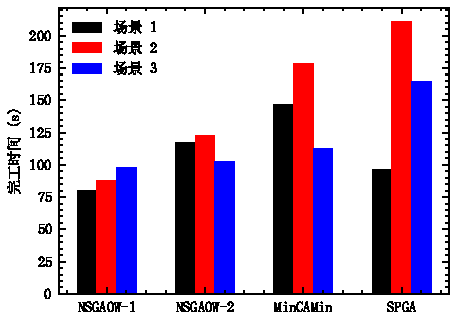
\includegraphics{img/min_secu_vs_makespan.pdf}
    \caption{不同隐私需求场景对完工时间的影响}
\end{figure}

在完工时间方面,本文发现不同优化侧重的算法有不同的差异:
优先优化完工时间的调度策略(NSGAOW-1和SPGA)在场景1中的完工时间低于场景3。例如,NSGAOW-1在场景1中的完工时间为80.15秒,低于场景3的98.17秒;SPGA在场景1中的完工时间为96.19秒,也低于场景3的129.77秒。这种现象与其优化目标密切相关:NSGAOW-1与SPGA优先优化完工时间,在场景1中尽可能利用公私云协作加速任务处理,而在场景3中,高安全性需求限制了公私云协作的使用,因此完工时间相对增加。
更关注成本与安全性的调度策略,如NSGAOW-2与MinCAMin,在场景3中的完工时间低于场景1。例如,NSGAOW-2在场景3中的完工时间为102.62秒,低于场景1的116.98秒;MinCAMin在场景3中的完工时间为132.72秒,也低于场景1的146.41秒。这是因为这两种算法优先使用私有云资源处理任务以提高安全性并降低成本。在场景1中,部分隐私数据可以进行公私云协作,但独立处理的任务会大量占用私有云资源,导致公私云协作效率下降,从而延长完工时间。而在场景3中,所有隐私数据均强制调度至私有云处理,私有云资源的集中利用反而提高了整体效率。

\section{加密计算开销对调度算法的影响}

在加密开销对调度算法的影响研究中,为了控制变量,实验固定隐私加密算法组中仅包含两条策略:一条是协作安全策略,即隐私数据经过加密后由公有云和私有云协作处理;另一条是私有云独立处理策略。实验在固定任务数量、数据大小等条件下,通过调整协作安全策略的加密开销来观察调度性能的变化。根据前文隐私加密算法组的加密开销范围,调整加解密开销的范围确定为50,200,350,500,650 CPU周期/bit。

\begin{figure}
    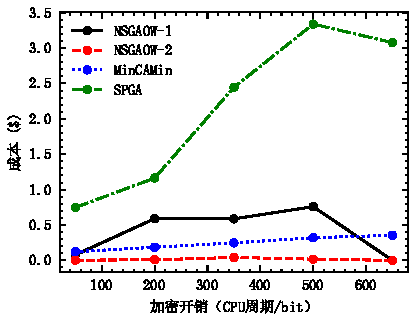
\includegraphics{img/enc_ovhd_vs_cost.pdf}
    \caption{不同加密开销对成本的影响}
\end{figure}

分析加密开销对成本的影响发现:首先,SPGA在成本方面表现最差,其在所有加密开销场景下的成本均显著高于其他算法。例如,当加密开销为500时,SPGA的成本为3.34元,而NSGAOW-2仅为0.02元。这主要是因为SPGA仅注重提升私有云利用率,未优化公有云租用策略,导致公有云资源利用率低下。此外,NSGAOW-1在多数场景下的成本高于NSGAOW-2,这是由于NSGAOW-1优先通过公私云协作降低完工时间,增加了公有云租用开销。然而,当加密开销达到650时,NSGAOW-1与NSGAOW-2的成本均趋近于零(分别为0.003元和0.001元),表明此时公私云协作对效率的贡献几乎消失。这是因为当加密开销接近或超过私有云直接处理的开销时,公私云协作无法进一步优化完工时间或成本,因此算法倾向于选择私有云处理隐私数据。基于这一发现,本文初步提出了一个判定隐私加密算法是否适用于混合云公私云协作的指标:加密开销小于直接计算的开销。最后,NSGAOW-2和MinCAMin在成本方面表现优异,这得益于二者均优先将任务调度至私有云处理,从而显著减少了公有云租用开销。

\begin{figure}
    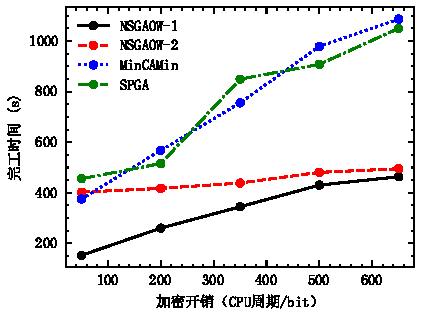
\includegraphics{img/enc_ovhd_vs_makespan.pdf}
    \caption{不同加密开销对完工时间的影响}
\end{figure}

% 论文格式修正,不要加粗,不要分列表,减少用括号表示

本节还分析了加密开销对完工时间的影响,发现随着加密开销的增加,所有算法的完工时间普遍呈现上升趋势。主要由额外的加密开销导致。其中,NSGAOW-2的完工时间增长幅度最低,这得益于其优先利用私有云空闲资源处理任务,从而降低了对加密开销的敏感性。例如,当加密开销从50增加到650时,NSGAOW-2的完工时间从402.52秒增至495.06秒,增幅仅为23\%,低于其他算法。此外,随着加密开销的增加,NSGAOW-1与NSGAOW-2的完工时间差值逐渐缩小。例如,在加密开销为50时,差值为249.74秒(NSGAOW-1为152.78秒,NSGAOW-2为402.52秒);而在加密开销为650时,差值缩小至31.63秒(NSGAOW-1为463.43秒,NSGAOW-2为495.06秒)。这种变化的原因与加密开销对成本的影响一致:随着加密开销的增加,公私云协作对完工时间的优化贡献逐渐减弱。当加密开销接近或超过私有云直接处理的开销时,公私云协作的收益显著降低,因此NSGAOW-1的完工时间趋近于NSGAOW-2。

\section{本章小结}

本章通过实验验证了所提出的混合云动态细粒度隐私任务调度模型与NSGA-OW多目标调度算法在任务调度中的性能表现。实验分为多目标优化性能、任务量与数据规模影响、隐私需求影响以及加密开销影响四个部分。首先,通过IGD和HV指标评估发现,NSGA-OW在收敛速度和解集质量上均优于对比算法,这一优势主要来自于针对混合云隐私任务调度问题所改进的遗传算子。其次,任务量与数据规模实验中发现,NSGA-OW算法在完工时间上降低了52.7\%,安全性提升了31.9\%,同时在成本上不劣于对比算法。随后,隐私需求对算法影响实验显示,NSGA-OW在不同隐私需求场景下均能有效平衡效率与安全,其在处理高隐私需求任务时表现尤为优秀。最后,加密计算开销实验表明,随着加密开销的增加,公私云协作对完工时间的优化贡献逐渐减弱。当加密开销接近或超过私有云直接处理的开销时,公私云协作的收益显著降低。本章实验结果说明,所提出的算法在收敛速度、解集质量及完工时间、安全性目标函数方面均优于对比算法。
